% Sample apostrophy's to remove team's 

\chapter{Introduction}
\label{IntroductionChapter}

Imagine that you are a Vice President of a multi-million dollar software development business unit managing 100 software engineers and 20 product managers. You have 25 teams working on various interrelated software products. The entire organization balances 1) adding new features to the next release, 2) solving customer escalations from installed products, and 3) handling maintenance chores such as routinely upgrading dependencies. Over the last few releases, you have seen a continuing decrease in your teams' productivity, and a steep increase in complaints from customers related to product quality. And somehow, there is never enough time to address those challenges.

In the middle of all this, one team is extremely difficult  to manage. The team is composed of highly skilled software engineers. They write well tested, clean code. The test suite is slow, but is thorough and catches issues before they get to the customer. 

The team resists collaborating with other teams or customers. The team developed an \quotes{us versus them} or \quotes{us versus management} attitude. Their product manager would like the team to be in the office more often to increase collaboration. While the organization expects teams to be in the office during core business hours, this team believes that as long as the work gets done, nobody should care where or when they accomplish the work. The product manager is growing frustrated with the team's attitude about features. Their focus appears to be on delivering something that works without truly understanding how the features should work. As a result, when they deliver code, the implementation does not always solve the customer's needs or works the way the customer expects. 

How did software development come to this? Why is software development so hard? Why is collaboration so difficult? How can we build teams that embrace collaboration, help others solve the problems, and train others to do their work?

The complexities of software development emerge, in part, due to 1) uncertainty about product to market fit resulting in changes to the feature set during and after development, 2) constantly changing dependent technologies, 3) the challenge of maintaining legacy code, 4) the lack of physical constraints resulting in boundless solutions, 5) measuring progress is challenging because project scope is a moving target and bringing visibility to an intangible process is difficult, and 6) software is written by people having various expertises as well as social and technical skills. Teams require coordination and collaboration. Building high performing teams requires effort and care. Unlike assembly line work, engineers are not fungible. Even if two engineers have the same competency in a set of technologies, their individual temperaments and personalities affect team dynamics. Building software is challenging. 

While it appears that any set of processes will work for tiny teams in the short term, creating an engineering culture where large teams deliver value week after week, month after month regardless of team disruption and changing circumstances is no easy task. Any company that achieves proficiency in software development becomes an interesting research opportunity. We choose Pivotal because it is successful; it is unusual in its continued use and evolution of Extreme Programming \cite{BeckExtremeProgramming2004};  it is accessible and cooperative with research. Chapter \ref{ResearchContextChapter} describes Pivotal, our research context. 

In order to understand how Pivotal develops software, we employed Constructivist Grounded Theory as the research method. Chapter \ref{ConstructivistGroundedTheoryChapter} describes Constructivist Grounded Theory and Chapter \ref{ResearchMethodChapter} describes our data sources and particular use of Grounded Theory. This study had an unusually ambitious scope. In many Grounded Theory studies, the researcher spends a few weeks interviewing participants and analyzing data. Here, one researcher spent \durationOfResearchStudyPlural{} working with participants 5 days per week on \numberOfObservedProjects{} teams. 

Applying Grounded Theory at Pivotal unearthed the theory of Sustainable Software Development, an explanation on how Pivotal teams can thrive despite team disruption and successfully deliver software to their stakeholders. Chapter \ref{SustainableSoftwareDevelopmentChapter} describes the theory's principles, policies, and practices. The theory explains how teams survive disruption by actively removing knowledge silos and caretaking the code. At the heart of the Pivotal process is team code ownership. Many of Pivotal's practices have the effect of promoting team code ownership while removing individual code ownership. Chapter \ref{TeamCodeOwnershipChapter} identifies five factors that affect the team's sense of code ownership and explains why psychological ownership causes some engineers to struggle with the transition from individual code ownership to team code ownership. 

The Grounded Theory study also identified that Pivotal teams actively detect and remove waste. Since software development is an organic and messy problem space, finding all kinds of waste is no surprise. Chapter \ref{SoftwareEngineeringWasteChapter} conducts the first empirical research study into a waste taxonomy and contrasts it with Lean Software Development's waste taxonomy. \sout{Some of the wastes types, such as \quotes{unnecessary cognitive effort,} are rarely salient unless one is specifically looking for them.}

Chapter \ref{ConclusionChapter} discusses future research and concludes the research study. 

Appendix \ref{AppendixChainOfEvidence} provides the chain of evidence for the waste taxonomy after iteratively applying constant comparison. 

Appendix \ref{AppendixInterviews} showcases interview data. The initial interviews began with the question, \quotes{draw your view of Pivotal's software development process.} The appendix includes a sample of these drawings with interview transcript snippets where the interviewee describes the drawing. Once team code ownership emerged as a core category, many interviews began with the question, \quotes{draw how you feel about the code.} Section \ref{AppendixFeelAboutTheCode} provides some of these drawings. When the pictures are not obvious, a brief narrative explains the illustration.

% opportunities to remove waste are apparent even for companies that actively remove waste. 

\chapter{Extreme Programming}
\label{ExtremeProgramming}

Kent Beck invented Extreme Programming while running the Chrysler payroll software project in 1996. \cite{BeckExtremeProgramming1999} In 1999, Beck published \underline{Extreme Programming Explained: Embrace Change}  \cite{BeckExtremeProgramming1999} and updated the it in 2004  \cite{BeckExtremeProgramming2004}. This chapter covers the latest version. 

Extreme programming balances business needs of repeatedly and reliably delivering software with the human needs of the participants. Extreme Programming is characterized by a set of values, principles, and practices. When transitioning a team to Extreme Programming, Beck recommends first adopting the primary practices. 
\section{Values}
Values help guide a team. Values remind a team why they do certain practices. Without values, a team might \quotes{cargo-cult} a practice (e.g. continue to religiously follow a practice without understanding why they follow it.) Beck says \quotes{values are the roots of the things we like and don't like in a situation} \cite{BeckExtremeProgramming2004}/ Values are abstract concepts, and hard to observe, whereas it is much easier to examine if a team is following a practice. \quotes{Practices are evidence of value \ldots Just as values bring purpose to practices, practices bring accountability to values} \cite{BeckExtremeProgramming2004}.

\textbf{Communication:} Extreme programming is a collaborative endeavor with frequent communication. Teams prefer open and transparent communication. 
\quotes{You can listen to people who have had similar problems in the past} \cite{BeckExtremeProgramming2004}. When combined with the reflective principle, the team can ask \quotes {what communication do you need to keep yourself out of this trouble in the future?} \cite{BeckExtremeProgramming2004}

\textbf{Simplicity:} Teams prefer simpler solutions to more complex solutions. Teams strive to \quotes{make a system simple enough to gracefully solve only today's problem} \cite{BeckExtremeProgramming2004}. Simpler solutions often take more work to discover and implement than complex solutions, but simpler solutions often require less communication than complex solutions.





\textbf{Feedback:} Feedback provides an opportunity for the team to respond to changing circumstances in the marketplace, in the product, in the team, and with the development process. Change requires feedback. In order for continuous improvement to work, the team decides to collect feedback at multiple frequencies and at multiple levels. The team prefers incremental improvement over expecting perfection. Teams attempt to shorten the feedback cycle so that the team can respond sooner rather than later.

\textbf{Courage:} \quotes{Courage is effective action in the face of fear}   \cite{BeckExtremeProgramming2004}. Sometimes it takes courage to make the needed change. Messy code will remain messy unless a programmer demonstrates courage to improve it. Individuals consider the consequences before making a change. With change, the team accepts the risk of unintended consequences (e.g. the tests fail.) When the team knows the problem, courage is a bias to action. When the team does not know the underlying problem, courage may simply be patience. 

\textbf{Respect:} Collaborative software development is founded on respect. Team members decide to respect each other. \quotes{If members of a team don't care about each other and what they are doing, XP won't work} \cite{BeckExtremeProgramming2004}.

\textbf{Others:} Teams may adopt additional values and align their practices around the values. 

\section{Principles}
The principles help guide a team in implementing the values. When two potential practices achieve the same value,  the principles guide the team. Beck shows that both documentation and daily conversations satisfy the need of communication, yet the principle of humanity reminds that daily communication satisfies the psychological need of human connection \cite{BeckExtremeProgramming2004}.

\textbf{Humanity:} The practices that a team follows need to satisfy human needs. Alternative software development practices may not respect psychological needs. A practice may grind away at an individual's humanity \cite{BeckExtremeProgramming2004}. Beck lists fundamental human needs as basic safety, accomplishment, belonging, growth, and intimacy \cite{BeckExtremeProgramming2004}. Team software development balances the needs of the individual with the needs of the team. 

\textbf{Economics:} The practices that a team follows need to balance business needs with technical needs\quotes. People buying the product fuels the business. {Software development is more valuable when it earns money sooner and spends money later} \cite{BeckExtremeProgramming2004}. Incremental design and incremental delivery allow the team to release earlier and delay expenses until later. Avoid building the illusive \quotes{perfect} product.

\textbf{Mutual Benefit:} The practices that a team follows need to find solutions that benefit everyone involved. A practice that does not benefit the team now is not mutually beneficial, e.g. writing documentation for a faceless, future maintenance team. Mutual beneficial practices help people now and in the future. 


\textbf{Self-Similarity:} The practices that a team follows can potentially be adapted to different contexts. Try applying solutions that work in one context to another context. Beck sees a similarity in listing themes for a quarter, addressing stories in a week, writing tests for a story.

\textbf{Improvement:} The practices that a team follows evolve and improve over time. Teams benefit from constant improvement. The point of XP is \quotes{excellence in software development through improvement} \cite{BeckExtremeProgramming2004}. Starting is preferred to waiting for perfection. 

\textbf{Diversity:} The practices that a team follows should resolve conflict productively. \quotes{Two ideas about a design present an opportunity, not a problem}  \cite{BeckExtremeProgramming2004}. Multiple perspectives provides richer solutions. Teams benefit from a diversity of skills, perspectives, attitudes, and experiences.

\textbf{Reflection:} The practices that a team follows should enable reflection at different frequencies and multiple levels. Teams reflect on how and why they are working. The team sees mistakes as opportunities for growth.

\textbf{Flow:} The practices that a team follows should decrease batch sizes to enhance flow. \quotes{Flow in software development is delivering a steady flow of valuable software by engaging in all the activities of development simultaneously}  \cite{BeckExtremeProgramming2004}. Teams want a steady stream of work moving through the system. The ideal \quotes{batch size} is one story per developer. Anything that interrupts the flow of work needs removing. 

\textbf{Opportunity:} The practices that a team follows need to frame problems as opportunities. A team \quotes{playing it safe} will make fewer mistakes but also move slower than needed.

\textbf{Redundancy:} The practices that a team follows should address difficult problems in multiple ways. \quotes{The critical, difficult problems in software development should be solved several different ways} \cite{BeckExtremeProgramming2004}. For example, XP handles the critical, difficult problem of defects with \quotes{pair programming, continuous integration, sitting together, real customer involvement, and daily deployment}  \cite{BeckExtremeProgramming2004}. 

% The team needs to continue in spite of team disruption. Spreading knowledge around the team helps it survive through churn. This enables people to go on vacation whenever needed.

\textbf{Failure:} The practices that a team follows prefer bias a team towards action. When the team does not know what to do, try something and get feedback. \quotes{If you're having trouble succeeding, fail} \cite{BeckExtremeProgramming2004}. Sometimes replacing lengthy conversation and debate with trying multiple ideas produces less waste.

\textbf{Quality:} The practices a team follows should deliver high-quality products. Increases in quality \quotes{leads to improvements in other desirable project properties, like productivity and effectiveness} \cite{BeckExtremeProgramming2004}. Beck argues that short-changing quality is not a way to make a project go faster. 

\textbf{Baby Steps:} The practices a team follows need to prefer small incremental changes. Start with the simplest smallest change possible and iterate from there. Decompose significant changes into small incremental changes. Beck often asks, \quotes {what's the least you could do that is recognizably in the right direction?} \cite{BeckExtremeProgramming2004}. 

\textbf{Accepted Responsibility:} The practices a team follows favors empowering people working on a problem the authority to solve it. Responsibility is accepted, not assigned. Avoid the situation where people in one part of the organization are telling others what to do. 

\section{Primary Practices}
For a team transitioning to Extreme Programming, Beck recommends starting with the primary practices. Beck claims that \quotes{the primary practices are useful independent of what else you are doing} resulting in an immediate improvement, whereas the corollary practices work well once a team has implemented the primary practices. Extreme programming is not dogmatic about the list of practices. The team chooses which practices to apply.

\begin{figure}[t]
\centering
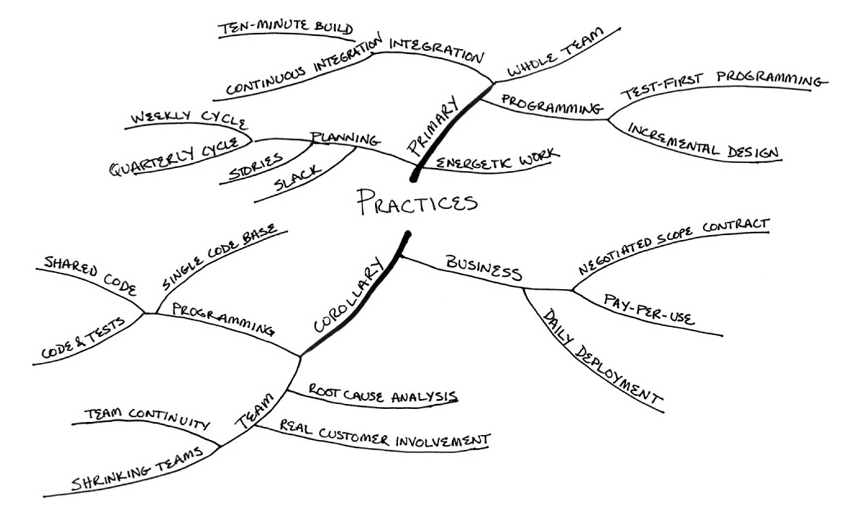
\includegraphics[width=\twoColumnWidth{}]{extreme_programming_images/summary_of_practices.png}
\caption{Extreme Programming Practices \cite{BeckExtremeProgramming2004}}
\label{XPSummaryOfPractices}
\end{figure}

\textbf{Sit Together:} Software development is a collaborative endeavor. Co-locating teams increases collaboration. Distributed teams are still possible, yet \quotes{Sit Together predicts that the more face time you have, the more humane and productive the project}  \cite{BeckExtremeProgramming2004}. 

%Synchronous communication enables a high bandwidth conversation, where participants can quickly discuss and iterate on a topic. Asynchronous communication (e.g. email or instant messaging) introduces delays in responses, context switching, the overhead of preparing a message, and increased opportunities for messages to be misunderstood. Co-locating the team into the same aisle increases the opportunities for synchronous communication and impromptu team huddles.  Co-located teams typically have greater verbal and nonverbal communication compared to distributed teams. Daily standups provide inexpensive touch points for the team to synchronize and resolve issues. Teams prefer synchronous communication over asynchronous communication. 

\textbf{Whole Team:} Whole team is also known as cross-functional teams. Include people on the team with the skills needed for success. Beck points out that a sense of team fulfills an individual's psychological needs. \quotes{We belong. We are in this together. We support each others' work, growth, and learning.} \cite{BeckExtremeProgramming2004}
 
%The entire team is responsible for the success of the project, and thus is empowered to make decisions to get it done.


\textbf{Informative Workspace:} \quotes{An interested observer should be able to walk into the team space and get a general idea of how the project is going in fifteen seconds} \cite{BeckExtremeProgramming2004}. The team can modify the workspace to make it more conducive for their work. 

% It should be possible to walk by the development area, and visible see the progress of the team. 

\textbf{Energized Work:} \quotes{Work only as many hours as you can be productive and only as many hours as you can sustain} \cite{BeckExtremeProgramming2004}. Working longer hours may make the team less productive. Team members need to take care of themselves; this includes staying home to rest when sick. The work patterns of the team should be sustainable in the long run.

\textbf{Pair Programming:} Every part of a production system is written by two programmers sitting side by side. The pair works together to solve problems, keep each other on task, learn from each other, and abide by the team's practices.

% Two engineers use one computer with two monitors, two keyboards, and two mice to implement each story. Ideally, the two enter into a state of flow where, at the end of the day, no one knows who wrote what. No individual ownership.

\textbf{Stories:} Stories are \quotes{units of customer-visible functionality}  \cite{BeckExtremeProgramming2004}. Stories have a name and a description or graphical depiction. Stories track the work to be done.

% The product manager decomposes a product into features and decomposes features into stories. Stories describe how the user interacts with the system.  Stories represent the unit of work to be done. Stories have acceptance criteria. 

\textbf{Weekly Cycle:} Each week, the team accepts a certain amount of work to accomplish. During a meeting at the beginning of the week, the team reviews progress to date, the customer chooses a week's worth of stories, and the engineers decompose the stories into tasks and individually estimate each task. \quotes{The goal is to have deployable software at the end of the week which everyone can celebrate as progress}  \cite{BeckExtremeProgramming2004}. 

% each engineer picks up a set of stories for the week. Engineers only estimate their stories to verify that they have enough capacity to accomplish the work for the week. Slack keeps slack for unforeseen circumstances.


\textbf{Quarterly Cycle:} Each quarter, the team identifies the stories for the next quarter.  During a meeting, the team identifies bottlenecks, initiates repairs, plans the feature sets for the quarter, and selects a quarter's worth of stories. 

% Each quarter, the team manager i. The product manager prioritizes the stories. The team plans for which features to implement during the next quarter.  A product roadmap is ...

\textbf{Slack:} During the weekly cycle meeting, include tasks in the plan that the team can drop if the team gets behind. Adding slack to the schedule enables a sustainable work environment.

\textbf{Ten-minute Build:} Building the code and running the test suite should be automated and short. Longer builds increase the feedback loop. 

\textbf{Continuous Integration:} When working on new features, routinely integrate new code into the master code repository. Avoid long-lived branches. Beck suggests un-integrated code live on its own \quotes{no more than a couple of hours}  \cite{BeckExtremeProgramming2004}.  The longer the team waits to integrate, the more unpredictable and expensive integration becomes. 

\textbf{Test-First Programming:} The developers write tests before writing code. Every production line of code is preceded by a test.  Test-first programming addresses several concerns: scope-creep,  coupling and cohesion, trust, and rhythm. The practice mitigates against scope-creep; without a clear goal, a programmer can easily write more code than is necessary. The practice improves coupling and cohesion as easy-to-test code often has beneficial design qualities. The practice builds trust in the code as engineers trust tested code more than un-tested code. The practice produces rhythm as it provides a cadence of accomplishing goals.

\textbf{Incremental Design:} Build the system incrementally and evolve the design every day. In the past, software teams might often had long design phases that assumed features would not change. When the team's understanding of the system changes, make incremental changes to the system to align the code's design with the team's desired goal. Routinely remove duplication.

\section{Corollary Practices}
Once a team has implemented the primary practices, then the team can start implementing the corollary practices. Beck says that it seems \quotes {difficult or dangerous to implement [the corollary practices] before completing the preliminary work of the primary practices} \cite{BeckExtremeProgramming2004}.

\textbf{Real Customer Involvement:} Make the customer a part of the team. \quotes{The point of customer involvement is to reduce wasted effort by putting the people with the needs in direct contact with the people who can fill those needs}  \cite{BeckExtremeProgramming2004}.

% The customer drives the feature selection, not the team.

\textbf{Incremental Deployment:} Switch between a legacy system and a replacement system in incremental steps. Avoid a hard switch over from a legacy system to a new system.

% Deliver code early and often.

\textbf{Team Continuity:} \quotes{Keep effective teams together}  \cite{BeckExtremeProgramming2004}. People are not fungible, and building relationships is part of creating a high performing team. Rotating people through teams helps spread knowledge.

\textbf{Shrinking Teams:} Try to improve team efficiency so that the team can shrink in size. When a team becomes more productive, re-allocated extraneous team members to other teams.

% Allocate people to where they are needed in the organization

\textbf{Root-cause analysis:} When a defect occurs, determine why it happened. Modify testing strategy to prevent that kind of mistake from happening again. Write an automated system test and an automated unit test then fix the code. 

\textbf{Shared Code:} Everyone on the team can modify any of the system. When engineers sees something broken, they fix it.

\textbf{Code and Tests:} The tests and code are the only permanent artifacts. Everything else (e.g. documentation) is generated from the code. Anything that contributes to what the system does today and what it will do tomorrow is valuable, \quotes{everything else is waste} 
\cite{BeckExtremeProgramming2004}.

\textbf{Single Code Base:} Ideally there is only one branch of the code. Multiple branches, (e.g. for releases, or customers) creates extra work. Branches live a few hours at most.

\textbf{Daily Deployment:} Every day put a new version of the code into production. 

\textbf{Negotiated Scope Contract:}  \quotes{Write contracts for software development that fix time, costs, and quality but call for an ongoing negotiation of the precise scope of the system.}

% Write contracts so that the client can re-prioritize the scope at any point in time, thus making the scope flexible.

\textbf{Pay-per-use:} Pay-per-use provides alignment between revenue and the features that generate the revenue. \quotes{Connecting money flow directly to software development provides accurate, timely information with which to drive improvement}  \cite{BeckExtremeProgramming2004}.


\section{Summary}

Every year VersionOne surveys the industry looking for trends in Agile software development \cite{VersionOne2016Report}. While surveys do have limitations, their data shows that many of the Extreme Programming practices are widely adopted by teams as shown in Figure \ref{VersionOne2016Practices}. One of the harder to adopt practices, pair programming is at 24\%. Pivotal provides a rare opportunity to study Extreme Programming in industry.


\begin{figure}[t]
\centering
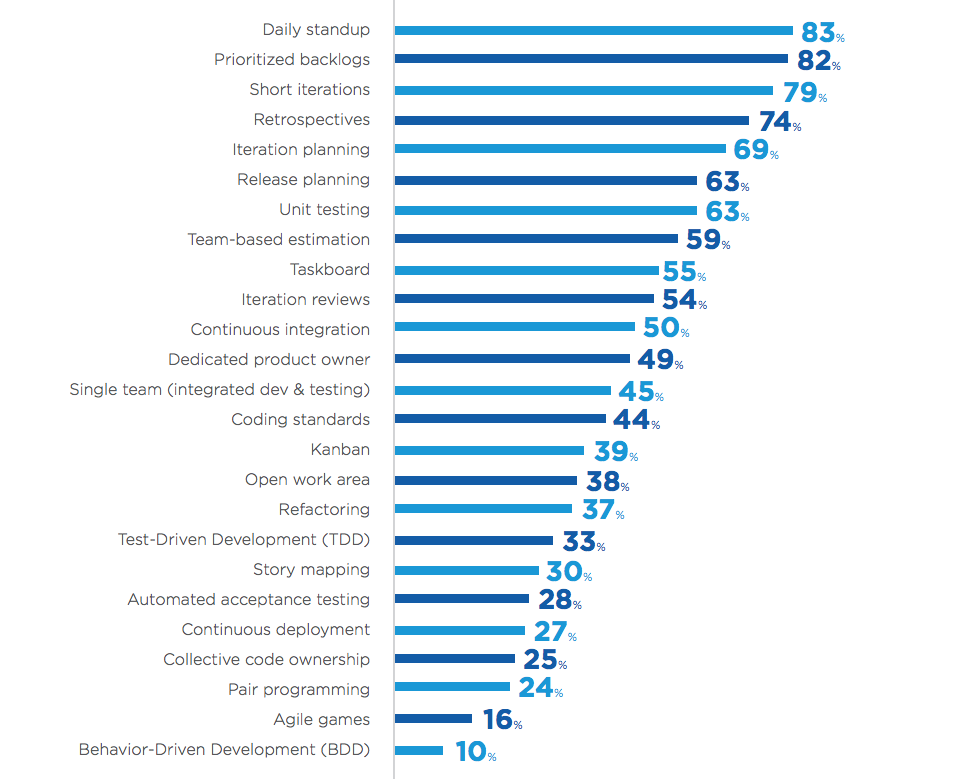
\includegraphics[width=\twoColumnWidth{}]{extreme_programming_images/version_one_2016_practices.png}
\caption{Agile Practices Adoption \cite{VersionOne2016Report}}
\label{VersionOne2016Practices}
\end{figure}

Extreme programming provides a collection of principles, values, and practices for adopting a balanced approach to software development. 


















\chapter{Research Context}
\label{ResearchContextChapter}

\section{Pivotal Labs}
Pivotal Labs is a division of Pivotal\textemdash a large American software company (with 17 offices around the world). Pivotal Labs provides teams of agile developers, product managers, and interaction designers to other firms. Its mission is not only to deliver highly-crafted software products but also to help transform clients' engineering cultures. To change the client's development process, Pivotal combines the client's software engineers with Pivotal's engineers at a Pivotal office where they can experience Extreme Programming \cite{BeckExtremeProgramming2004} in an environment conducive to agile development. 

Typical teams include six developers, one interaction designer, and a product manager. The largest project in the history of the Palo Alto office had 28 developers while the smallest had two. Larger projects are organized into smaller coordinating teams with one product manager per team and one or two interaction designers per team.

Interaction designers identify user needs predominately through user interviews; create and validate user experience with mockups; determine the visual design of a product; and support engineering during implementation. Product managers are responsible for identifying and prioritizing features, converting features into stories, prioritizing stories in a backlog, and communicating the stories to the engineers. Software engineers implement the solution. 

Pivotal Labs has followed Extreme Programming \cite{BeckExtremeProgramming2004} since the late 1990's. While each team autonomously decides what is best for each project, the company culture strongly suggests following all of the core practices of Extreme Programming, including pair programming, test-driven development, weekly retrospectives, daily stand-ups, a prioritized backlog, and team code ownership. We only observed teams at Pivotal Labs. Other teams, especially teams in other divisions, might have a different culture and follow different software practices.

\section{Day in the Life}
This section presents a typical day in the life of a Pivotal software engineer.

Pivotal provides breakfast to promote engineers starting the day at the same time. Many engineers socialize with their coworkers while eating breakfast. 

Office stand-up begins at 9:06 am \cite{BBCPivotal9am}. Everyone gathers around in a large circle. The stand-up covers \quotes{new faces,} \quotes{helps,} \quotes{interestings,} and \quotes{events.} The office stand-up lasts a few minutes. The two people running stand-up send an email to the company with a summary of the brief meeting. People then disperse for their team's stand-ups.

Team stand-ups provide a synchronization point for the team. Small teams (under eight people) typically will review what each individual accomplished yesterday and discuss any blockers to finishing the work. Large teams discuss \quotes{interestings} and \quotes{helps.} Some teams use a whiteboard to track \quotes{parking lot} issues (items needing discussion during stand-up). After team stand-up, the engineers then decide \quotes{pairing.} For work in progress, each pair decides who will continue with it. The available engineers then re-pair with engineers continuing the work. If a pair has nothing to work on, they take the next story at the top of the backlog. The team then determines which pairs will use which computer. If there is work already in progress on one machine, the pair continues the work on the same machine. The team configures the development environments to be identical on all machines. Pairing continues until 12:30 pm when the team takes a lunch break. After lunch, pairing continues until 6:00 pm. 

While coding, the developers follow Test Driven Development (or Behavior Driven Development.) Tests are written first before determining the design or writing code. A failing test provides the developers with a short term goal. The rhythm is to start a story, refactor if necessary, write a small failing test, write just enough code to get the test to pass, refactor if necessary, and repeat by writing a small failing test. The ideal flow is quick, short cycles of Test Driven Development. When a pair finishes their work, they start the next story at the top of the backlog. 

The interaction designer validates product features with user research, creates mock-ups of the user interaction, and validates mock-ups and the implemented product with users. After validating the mock-ups, the product manager converts the new feature into a set of small stories. Each story represents a small piece of interaction between the user and the system. By decomposing a feature into granular stories, the product manager can identify high value work to start now and delay low value work.  

The product manager determines the features and the sequence of stories. The prioritization is kept in a backlog. The product manager decides \quotes{what} the product should do. The engineers determine the implementation details, \quotes{how} the code should be written to accomplish the task in the story. The product manager changes the direction of the product at any point in time by resequencing the backlog. The product manager does not change any \quotes{in-flight} stories (stories that the developers are working on).

During each week, the team holds an iteration planning meeting. The product manager and designer communicate to the engineers the upcoming work, building a shared understanding of the stories. The engineers communicate to the product manager the complexity and risk associated with each story.

At the end of each week, the team holds a retrospection meeting to examine what is working well for the team, what needs improvement, and determine any action items to accomplish the identified improvements.


